% Notas:
% Sobre originalidad: distiguir mi software del SaaS
% ======================================

\section{Marco conceptual}

\subsection{Ingeniería de rendimiento de software (\emph{Software Performance Engineering})}
Una definición comúnmente utilizada para definir ingeniería de rendimiento de software  (\emph{Software Performance Engineering} - SPE)  es la que brinda en Woodside et al. \cite{4221619}: \textit{``Ingeniería de rendimiento de software representa toda la colección de actividades de ingeniería de software y análisis relacionados utilizados a través del ciclo de desarrollo de software que están dirigidos a cumplir con los requisitos de rendimiento''}. 

De acuerdo con este mismo autor, los enfoques para ingeniería de rendimiento puede ser divididos en dos categorías: basadas en mediciones y basadas en modelos. La primera es la más común y utiliza pruebas, diagnóstico y ajustes una vez que existe un sistema en ejecución que se puede medir, es por esto que solamente puede ser utilizada conforme se va acercando el final del ciclo de desarrollo de software. Al contrario del enfoque basado en mediciones, el enfoque basado en modelos se centra en las etapas iniciales del desarrollo. Como el nombre lo indica, en este enfoque los modelos son clave para hacer predicciones cuantitativas de qué tan bien una arquitectura puede cumplir sus expectativas de rendimiento.

Se han propuesto otras clasificaciones de enfoques para SPE pero, con respecto a la evaluación de sistemas basados en componentes, en \cite{Koziolek:2010:PEC:1808359.1808729} se deja la clasificación a un lado debido a que se argumenta que la mayoría de enfoques de modelaje toman alguna medición como entrada y a la mayoría de los métodos de medición los acompaña algún modelo.

\subsubsection{Ingeniería de rendimiento basada en mediciones}
Los enfoques basados en mediciones son los que prevalencen en la industria\cite{Gooijer2011PerformanceMO} y son típicamente utilizados para verificación(¿el sistema cumple con su requisito de rendimiento?) o para localizar y arreglar \emph{hot-spots} (cuáles son las partes que tienen peor rendimiento en el sistema). La medición de rendimiento se remonta al inicio de la era de la computación, lo que ha generado una amplia gama de herramientas como generadores de carga y monitores para crear cargas de trabajo ficticias y llevar a cabo la medición de un sistema respectivamente.

Las pruebas de rendimiento aplican técnicas basadas en medición y usualmente esto es hecho luego de las pruebas funcionales o de carga. Las pruebas de carga verifican el funcionamiento de un sistema bajo cargas de trabajo pesadas, mientras que las pruebas de rendimiento son usadas para obtener datos cuantitativos de características de rendimiento, como tiempos de respuesta, \emph{throughput} y utilización de hardware para una configuración de un sistema bajo una carga de trabajo definida.

\subsubsection{Ingeniería de rendimiento por medio de modelado} 
La importancia del modelado del rendimiento está motivada por el riesgo a que se presenten problemas graves de rendimiento y la creciente complejidad de sistemas modernos, lo que hace difícil abordar los problemas de rendimiento al nivel de código\cite{Reussner:2016:MSS:3036121}. Cambios considerables en el diseño o en las arquitecturas pueden ser requeridos para mitigar los problemas de rendimiento. Por esta razón, la comunidad de investigación de modelado de rendimiento intenta luchar contra el enfoque de ``arreglar las cosas luego'' durante el proceso de desarrollo. Con la aplicación de un modelo del rendimiento de software se busca encontrar problemas de rendimiento y alternativas de diseño de manera temprana en el ciclo de desarrollo, evitando así el costo y la complejidad de un rediseño o cambios en los requerimientos.

Las herramientas de modelado de rendimiento ayudan a predecir la conducta del sistema antes que este sea construido o bien, evaluar el resultado de un cambio antes de su implementación. El modelado del rendimiento puede ser usado como una herramienta de alerta temprana durante todo el ciclo de desarrollo con mayor precisión y modelos cada vez más detallados a lo largo del proceso. Al inicio del desarrollo un modelo no puede ser validado contra un sistema real, por esto el modelo representa el conocimiento incierto del diseñador. Como consecuencia de esto el modelo hace suposiciones que no necesariamente se van a dar en el sistema real, pero que van a ser útiles para obtener una abstracción del comportamiento del sistema. En estas fases iniciales, la validación se obtiene mediante el uso del modelo, y existe el riesgo de conclusiones erróneas debido a su precisión limitada. Luego, el modelo puede ser validado contra mediciones en el sistema real (o parte de este) o prototipos y esto hace que la precisión del modelo se incremente.

En \cite{Jin:2007:PEP:1248820.1248885} se sugiere que los métodos actuales tienen que superar un número de retos antes que puedan ser aplicados en sistemas existentes que enfrentan cambios en su arquitectura o requerimientos. Primero, debe quedar claro cómo se obtienen los valores para los parámetros del modelo y cómo se pueden validar los supuestos. Estimaciones basadas en la experiencia para estos parámetros no son suficientes y mediciones en el sistema existente son necesarias para hacer predicciones precisas. Segundo, la caracterización de la carga del sistema en un entorno de producción es problemática debido a los recursos compartidos (bases de datos, hardware). Tercero, deben desarrollarse métodos para capturar parámetros del modelo dependientes de la carga. Por ejemplo un incremento en el tamaño de la base de datos probablemente incrementará las necesidades de procesador, memoria y disco en el servidor.

Técnicas comunes de modelado incluyen redes de colas y también extensiones de estas como redes de colas en capas y varios tipos de redes de Petri, y procesos de álgebra estocástica.

\subsubsection{Modelado de Rendimiento}
En SPE, la creación y evaluación de modelos de rendimiento es un concepto clave para evaluar cuantitativamente el rendimiento del diseño de un sistema y predecir el rendimiento de otras alternativas de diseño. Un modelo de rendimiento captura el comportamiento relevante al rendimiento de un sistema para identificar el efecto de cambios en la configuración o en la carga de trabajo en el rendimiento. Permite predecir los efectos de tales cambios sin necesidad de implementación y ejecución en un ambiente de producción, que podrían ser no solamente tareas costosas sino también un desperdicio en el caso que un el hardware con el que se cuenta pruebe ser insuficiente para soportar la intensidad de la carga de trabajo.\cite{Noorshams2015_1000046750}

La forma del modelo de rendimiento puede comprender desde funciones matemáticas a formalismos de modelado estructural y modelos de simulación. Estos modelos varían en sus características clave, por ejemplo, las suposiciones de modelado de los formalismos, el esfuerzo de modelado requerido y el nivel de abstracción.

En cuanto a técnicas de simulación, a pesar que estas permiten un estudio más detallado de los sistemas que modelos analíticos, la construcción de un modelo de simulación requiere de conocimiento detallado tanto de desarrollo de software como de estadística\cite{Gooijer2011PerformanceMO}. Los modelos de simulación también requieren usualmente de mayor tiempo de desarrollo que los modelos analíticos. En \cite{4221619} se menciona que ``la construcción de un modelo de simulación es caro, algunas veces comparable con el desarrollo de un sistema, y, los modelos de simulación detallados puede tardar casi tanto en ejecutarse como el sistema''.

\subsection{Modelado y simulación de rendimiento basado en componentes}
En este enfoque, modelos clásicos de rendimiento tales como redes de colas, redes de Petri estocásticas o procesos de álgebra estócastica son aplicados para modelar y analizar el rendimiento de software basado en componentes. La ingeniería de software basada en componentes se considera un sucesor del desarrollo de software orientado a objetos, en esta los componentes de software son unidades de composición a las que se le define una especificación y una interfaz. A partir de estas, los arquitectos de software construyen e integran componentes de software entre sí, creando de esta manera sistemas más complejos.\cite{Koziolek:2010:PEC:1808359.1808729}

El reto en los modelos de rendimiento para componentes, es que el rendimiento de un componente de software en un sistema en ejecución depende del contexto en que está instlado y su perfil de uso, el cual es usualmente desconocido por el desarrollador del componente que creal el modelo de un componente individual.

\subsubsection{Rendimiento de componentes de software}
Szyperski\cite{Szyperski:2002:CSB:515228} define un componente de software como: \textit{``Un componente es una unidad de composición en aplicaciones de software, que posee un conjunto de interfaces y un conjunto de requisitos (una especificación), y que ha de poder ser desarrollado, adquirido, incorporado al sistema y compuesto con otros componentes de forma independiente, en tiempo y espacio''}. 

Los componentes de software presentan los principios de ocultación de la información y la separación de responsabilidades. Fomentan la reutilización y preparan el sistema para que se puedan efectuar cambios de partes individuales. Permiten además una división de trabajo entre los desarrolladores de componentes y los arquitectos de software, lo que reduce la complejidad de la tarea de desarrollo. Los componentes de caja negra (\emph{black-box}) solamente revelan sus interfases a los clientes, mientras que los componentes de caja blanca (\emph{white-box}) permiten ver y modificar el código fuente de la implementanción del componente como tal. Los componentes compuestos agrupan varios componentes en unidades más grandes.

\paragraph{Factores que influyen el rendimiento de un componente}
Especificar el rendimiento de componentes reutilizables es difícil porque esto no solamente va a depender de la implementación del componente, sino también del contexto en donde se encuentre instalado. Los factores que influyen en el rendimiento de los componentes son:

\begin{figure}[h]
  \centering
  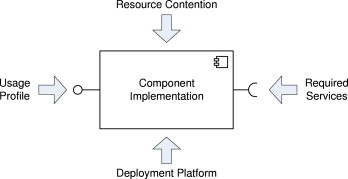
\includegraphics[width=10cm]{component-performance}
  \caption[Factores que influyen en el rendimiento de un componente]{Factores que influyen en el rendimiento de un componente. Tomado de \protect\cite{Koziolek:2010:PEC:1808359.1808729}}
  \label{fig:component-performance}
\end{figure}

\begin{itemize}
    \item \emph{Implementación del componente}: los desarrolladores pueden implementar la funcionalidad especificada en una interfaz de diferentes formas. Dos componentes pueden proporcionar el mismo servicio pero presentar tiempos de ejecución diferentes cuando se ejecutan con los mismos recursos y con las mismas entradas.
    \item \emph{Servicios requeridos}: cuando el componente $A$ invoca el servicio del componente $B$, el tiempo de ejecución de $B$ suma al tiempo de ejecución de $A$. Por lo tanto, el tiempo total de ejecución de un componente depende del tiempo de ejecución de los otros componentes/servicios que necesita.
    \item \emph{Plataforma de instalación}: los arquitectos de software instalan un componente de software en diferentes plataformas. Una plataforma de instalación puede incluir varias capas de software (como por ejemplo contenedores de componentes o máquinar virtuales) y hardware (procesador, dispositivos de almacenamiento y red, etc)
    \item \emph{Perfil de uso}: clientes pueden invocar los servicios del componente con diferentes parámetros de entrada. El tiempo de ejecución de un servicio puede cambiar dependiendo de los valores de lo parámetros de entrada.
    \item \emph{Contención de recursos}: un componente de software típicamente no se ejecuta como un solo proceso aislado en una plataforma determinada. Los tiempos de espera inducidos para acceder a recursos limitados se suman al tiempo de ejecución de un componente de software.
\end{itemize}

\subsubsection{Enfoques de ingeniería de rendimiento para software basado en componentes propuestos}
La encuesta llevada a cabo en \cite{Koziolek:2010:PEC:1808359.1808729} proporciona una clasificación de enfoques de medición y predicción de rendimiento para sistemas de software basados en componentes. Otra clasificación es la que se expone en \cite{1291833} donde se presenta una revisión de métodos de predicción de rendimiento basado en modelos para sistemas en general, pero no analiza los requerimientos propios para sistemas basados en componentes. 

De acuerdo con \cite{Koziolek:2010:PEC:1808359.1808729} durante los últimos diez años, los investigadores han propuesto muchos enfoques para evaluar el rendimiento (tiempos de respuesta, \emph{throughput}, utlización de recursos) de sistemas de software basados en componentes. Estos enfoques abarcan tanto predicción como medición del rendimiento. Los primeros analizan el rendimiento esperado de un diseño de software basado en componentes para evitar problemas de rendimiento en la implementación del sistema, lo que podría llevar a costos substanciales para rediseñar la arquitectura. Los otros analizan el rendimiento observable de sistemas de software basados en componentes implementados para entender sus propiedades, determinar su capacidad máxima, identificar componentes críticos y para remover cuellos de botella.

\paragraph{Métodos de evaluación de rendimiento}
Los enfoques se agruparon en dos grandes grupos: enfoques principales que proporcionan procesos de evaluación de rendimiento completo y enfoques suplementarios que se centran en aspectos específicos como medición de componentes individuales o modelaje de las propiedades de rendimiento de los conectores de un componente.

\paragraph{Enfoques principales}
\begin{itemize}
    \item \textbf{Enfoques de predicción basados en UML}: los enfoques en este grupo se enfocan en la predicción de rendimiento en tiempo de diseño para sistemas de software basado en componentes modelados con el Lenguaje de Modelado Unificado (UML por sus siglas en inglés). UML 2.0 tiene la noción de componente de software como una clase extendida. UML permite modelar el comportamiento de un un componente con diagramas de sequencia, actividad y colaboración. El alojamiento de los componentes puede ser descrito como con diagramas de despliegue(\emph{deployment}).     
%    Mientras que UML solamente soporta especificaciones funcionales, su mecanismo de extensión (perfiles que consisten de estereotipos, restricciones y valores etiquetados) ha sido utilizado por el \emph{Object Management Group} para permitir el modelado de atributos de rendimiento como valores de tiempo y parámetros de cargas de trabajo. 
    \begin{itemize}
        \item CB-SPE - \emph{Component-Based Software Performance Engineering} 
    \end{itemize}
    \item \textbf{Enfoques de predicción basados en Meta-Modelos propietarios}: Los enfoques en este grupo apuntan a las predicciones de rendimiento de tiempo de diseño. En lugar de usar UML como lenguaje de modelado para desarrolladores y arquitectos, estos enfoques tienen meta-modelos propietarios.
    \begin{itemize}
        \item CBML - \emph{Component-Based Modeling Language}
        \item PECT - \emph{The Prediction Enabled Component Technology}
        \item COMQUAD - \emph{Components with Quantitative properties and Adaptivity}
        \item KLAPPER
        \item ROBOCOP
        \item Palladio        
    \end{itemize}
    \item \textbf{Enfoques de predicción centrados en \emph{middleware}}: hacen énfasis en la influencia del \emph{middleware} en el rendimiento de un sistema basado en componentes. Por lo tanto miden y modelan el rendimiento de plataformas \emph{middleware} como JavaEE o .Net. Se basan en la suposición que la lógica de negocio de los componentes como tal tienen poco impacto en el rendimiento general del sistema y por eso no requieren un modelado detallado.
    \begin{itemize}
        \item NICTA
    \end{itemize}
    \item \textbf{Enfoques basados en especificaciones formales}: estos enfoques siguen teorías fundamentales de especificación de rendimiento y no toman en cuenta marcos de trabajo (\emph{frameworks}) de medición y predicción.
    \begin{itemize}
        \item RESOLVE
        \item HAMLET
    \end{itemize}
    \item \textbf{Enfoques de monitoreo para sistemas implementados}: asumen que un sistema basado en componentes ha sido implementado y puede ser probado. El objetivo es encontrar problemas de rendimiento en un sistema en ejecución, identificar cuellos de botella y adaptar el sistema para que pueda lograr los requerimientos de rendimiento.
   \begin{itemize}
        \item COMPAS
        \item TESTEJB
        \item AQUA
        \item PAD
    \end{itemize}    
\end{itemize}
  

\paragraph{Enfoques Suplementarios}
\begin{itemize}
    \item \textbf{Enfoques de monitoreo para componentes implementados}: El objetivo de los enfoques de medición para implementaciones de componentes de software individuales es derivar especificaciones de rendimiento parametrizadas a través de mediciones múltiples. El objetivo es obtener el perfil de uso, dependencias y la plataforma de implementación a partir de la especificación de rendimiento, de modo que pueda usarse en diferentes contextos. 
    \begin{itemize}
        \item RefCAM
        \item COMAERA
        \item ByCounter
    \end{itemize}
    \item \textbf{Enfoques de predicción con énfasis en conectores de componentes}: Estos enfoques asumen un lenguaje de descripción de componentes existente y se centran en modelar y medir el impacto en el rendimiento de las conexiones entre componentes. Estas conexiones pueden implementarse con diferentes técnicas \emph{middleware}.
    \begin{itemize}
        \item Verdickt
        \item Grassi
        \item Becker
        \item Happe
    \end{itemize}        
\end{itemize}

Recientemente varios enfoques de predicción basados en meta-modelos propietarios han sido propuestos para optimización de diseño de arquitecturas, modelado de calidad de servicio y escalabilidad. PerOpteryx\cite{Koziolek:2011:PAA:2000259.2000267} es un enfoque de optimización de diseño de arquitecturas que manipula modelos especificados en \emph{Palladio Component Model}\cite{Reussner:2016:MSS:3036121} y utiliza el algoritmo evolutivo multi-objetivo \texttt{NSGA-II}. Para análisis de rendimiento utiliza redes de colas en capas. \emph{Descartes Modeling Language}\cite{KoBrHu2014-TechReport-DML} es un lenguaje de modelado de arquitecturas para modelar calidad de servicio y aspectos relacionados con la gestión de recursos de los sistemas, las infraestructuras y los servicios de tecnología de información dinámicos modernos. \emph{CloudScale}\footnote{\url{http://www.cloudscale-project.eu/}}\cite{Brataas:2013:CSM:2479871.2479920} es un enfoque de diseño y evolución de aplicaciones y servicios escalables en la nube. En \emph{CloudScale} se identifica y gradualmente se resuelven problemas de escalabilidad en aplicaciones existentes y también permite el modelado de alternativas de diseño y el análisis del efecto de la escalabilidad en el costo. Cabe mencionar que estos últimos enfoques han sido influenciado en gran medida por el trabajo llevado a cabo en \emph{Palladio Component Model}.

\subsubsection{Modelado de Arquitecturas de Software con \emph{Palladio Component Model}} \label{sec:pcm}
El \emph{Palladio Component Model} es un enfoque de modelaje para arquitecturas de software basados en componentes que permite predicción de rendimiento basada en modelos. PCM contribuye el proceso de desarrollo de ingeniería basado en componentes y proporciona conceptos de modelaje para describir componentes de software, arquitectura de software, despliegue (\emph{deployment}) de componentes y perfiles de uso de sistemas de software basados en componentes en diferentes submodelos (Figura \ref{fig:pcm-instance}). 

\begin{figure}[h]
  \centering
  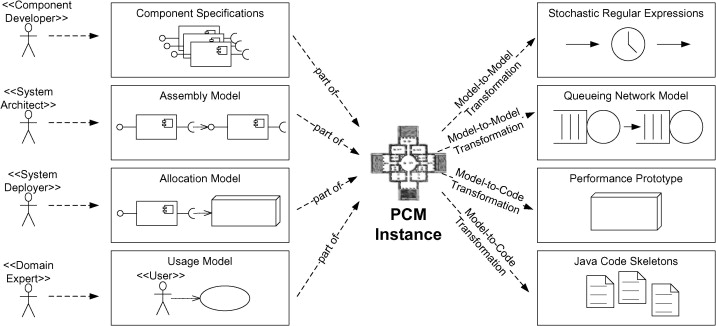
\includegraphics[width=15cm]{palladio-cbse-process}
  \caption[Instancia de un modelo PCM]{Instancia de un modelo PCM. Tomado de \protect\cite{Becker:2009:PCM:1458724.1458819}}
  \label{fig:pcm-instance}
\end{figure}

\begin{itemize}
    \item \textbf{Especificaciones de componentes} son descripciones abstractas y paramétricas de los componentes de software. En las especificaciones de software se proporciona una descripción del comportamiento interno del componente así como las demandas de sus recursos en RDSEFFs (\emph{Resource Demanding Service EFFect specifications}) utilizando una sintaxis similar a los diagramas de actividad de UML.
    \item \textbf{Un modelo de ensamblaje} (\emph{assembly model}) especifica qué tipo de componentes se utilizan en una instancia de aplicación modelada y si las instancias del componente se replican. Además, define cómo las instancias del componente se conectan representando la arquitectura de software.
    \item El entorno de ejecución y los recursos, así como la instalación (\emph{deployment}) de instancias de componentes para dichos contenedores de recursos se definen en un \textbf{modelo de asignación} (\emph{allocation model}).
    \item El \textbf{modelo del uso} especifica la interacción de los usuarios con el sistema utilizando una sintaxis similar al diagrama de actividades de UML proporcionando una descripción abstracta de la secuencia y la frencuencia en que los usuarios activan las operaciones disponibles en un sistema.
\end{itemize}

Un modelo PCM abstrae un sistema de software a nivel de arquitectura y se anota con consumos de recursos que fueron medidos previamente u otros que son estimados. El modelo puede entonces ser usado en transformaciones de modelo-a-modelo o modelo-a-texto a un modelo de análisis en particular (redes de colas o simulación de código) que puede ser analíticamente resuelto o simulado para obtener resultados sobre el rendimiento y predicciones del sistema modelado. Los resultados del rendimiento y las predicciones pueden ser utilizadas como retroalimentación para evaluar y mejorar el diseño inicial, permitiendo así una evaluación de calidad de los sistemas de software en base a un modelo\cite{Noorshams2015_1000046750}.


\subsubsection{Modelado de Arquitecturas de Software con \emph{Descartes Modeling Language}} \label{sec:dml}
El \emph{Descartes Modeling Language} (DML) es un lenguaje de modelado a nivel de arquitectura utilizado para describir calidad de servicio (\emph{QoS} por sus siglas en inglés) y aspectos relacionados con la gestión de recursos de sistemas de información dinámicos, infraestructuras y servicios. DML distingue explicítamente diferentes tipos de modelos que describen el sistema y sus procesos de adaptación desde un punto de vista técnico y lógico. Juntos, estos diferentes tipos de modelos forman una instancia DML. La idea detrás del uso de estos modelos es separar el conocimiento acerca de la arquitectura del sistema y el comportamiento de su rendimiento (aspectos técnicos) del conocimiento de los procesos de adaptación del sistema (aspectos lógicos)\cite{KoBrHu2014-TechReport-DML}.

\begin{figure}[h]
  \centering
  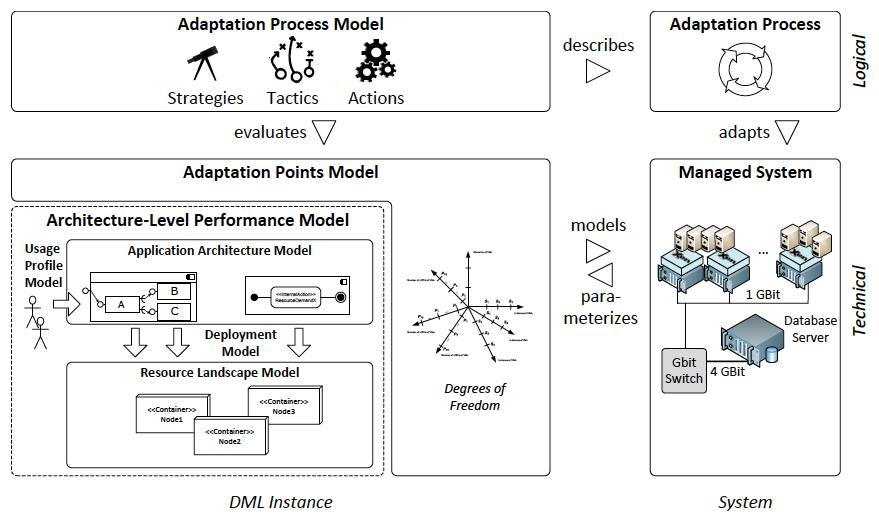
\includegraphics[width=16cm]{dml-instance}
  \caption[Relación de los diferentes modelos de una instancia DML y el sistema]{Relación de los diferentes modelos de una instancia DML y el sistema. Tomado de \protect\cite{KoBrHu2014-TechReport-DML}}
  \label{fig:dml-instance}
\end{figure}

La figura \ref{fig:dml-instance} muestra la relación de los diferentes modelos que son parte de una instancia DML, el sistema gestionado (\emph{managed system}) y el proceso de adaptación del sistema (\emph{adaptation process}). En la esquina inferior derecha de la figura \ref{fig:dml-instance}, se ve el sistema, el cual es gestionado por un proceso de adaptación, mostrado en la esquina superior derecha de la figura \ref{fig:dml-instance}. En la esquina inferior izquierda de, se muestran modelos que reflejan los aspectos técnicos del sistema. Esos aspectos son los recursos de hardware y su distribución (\emph{resource landscape model}), los componentes de software y el comportamiento relevante al rendimiento (\emph{application architecture model}), la instalación de componentes de software en el hardware (\emph{deployment model}), el comportamiendo del uso y las cargas de trabajo de los usuarios del sistema (\emph{usage profile model}) y los grados de libertad del sistema que pueden ser empleados para la adaptación del sistema en ejecución (\emph{adaptation points model}). Por encima de estos modelos (esquina superior izquierda de la figura \ref{fig:dml-instance}) se muestra el modelo de proceso de adaptación que especifica un proceso de adaptación que describe cómo el sistema se adapta a cambios en su ambiente. El proceso de adaptación aprovecha las técnicas de predicción de rendimiento en línea para razonar sobre posibles estrategias, tácticas y acciones de adaptación.
 
\subsection{Computación en nube}
%La computación en la nube ha traído consigo nuevos estilos en la forma en cómo se desarrolla y se pone en producción el software. Esto motivado por ... \textbf{[EXTENDER]}

Según el NIST\cite{Mell:2011:SND:2206223}, el \emph{Cloud Computing}, o la Computación en la Nube, es un modelo que, desde la perspectiva del consumidor, permite el acceso conveniente, por demanda, desde alguna red, a un conjunto de recursos computacionales específicos y configurables (por ejemplo, redes, servidores, almacenamiento, aplicaciones y servicios) que pueden ser rápidamente provisionados y entregados con un esfuerzo mínimo de administración o de interacción con el proveedor del servicio.

\subsubsection{Modelos de entrega de servicio}

La definición del NIST presenta 3 modelos básicos de servicio. Aunque los proveedores de servicios de Cloud han creado muchas variaciones de ofertas \emph{``as-a-Service''}, estos 3 siguen siendo considerados los fundamentales.

\paragraph{Software como Servicio (SaaS)}
El cliente usa una aplicación, que se ofrece como un servicio accedido remotamente con protocolos estandarizados, pero no controla el sistema operativo, los servidores de aplicación, el hardware o la infraestructura de red en la que opera. El proveedor instala, administra y mantiene el software. El proveedor no necesariamente es dueño de la infraestructura física donde el software se está ejecutando. En general, se puede considerar un servicio para usuarios finales.

\paragraph{Plataforma como Servicio (PaaS)}
El cliente usa un sistema hospedado para sus aplicaciones. El cliente controla las aplicaciones que ejecuta en el ambiente (y posiblemente tenga algún control sobre el ambiente de hospedaje), pero no tiene acceso ni controla el sistema operativo, el hardware o la infraestructura de red donde ellas se ejecutan. La plataforma es típicamente un marco de ejecución aplicativo. El proveedor administra la infraestructura de software de la nube para la plataforma. En este caso, el cliente por lo general es un desarrollador de software.

\paragraph{Infraestructura como Servicio (IaaS)}
El cliente utiliza recursos computacionales fundamentales como poder de procesamiento, almacenamiento, comunicaciones y \emph{middleware}. El cliente puede controlar el sistema operativo, el almacenamiento, implementar aplicaciones y posiblemente algunos componentes de red como cortafuegos (\emph{firewalls}) y balanceadores de carga, pero la infraestructura física de red y de hardware no le pertenece. Los clientes habituales de estos servicios son administradores de sistemas.

\subsubsection{\emph{Serverless y Function-as-a-Service}}
FaaS es un área de lo que hoy se conoce como computación sin servidores o \emph{serverless computing}. Amazon.com, uno de los principales propulsores de esta tendencia define \emph{serverless} como una tecnología la cual permite construir y ejecutar aplicaciones y servicios sin necesidad de pensar en los servidores. Las aplicaciones \emph{serverless} no requieren de aprovisionamiento, escalamiento y administración de ningún servidor. Se puede construir con ella casi cualquier tipo de aplicación o servicio, y todo lo que se requiere para ejecutar y escalar la aplicación con alta disponibilidad es gestionado por el proveedor del servicio\cite{amazon:serverless-definition}. 

FaaS se refiere a un tipo de aplicación \emph{serverless} en donde la lógica del lado del servidor es escrita por un desarrollador pero, a diferencia de arquitecturas tradicionales, esta se ejecuta en contenedores de cómputo que no mantienen estado, son activados por medio de eventos, son efímeros (pueden durar solo una invocación) y son totalmente administrados por un tercero\cite{mike-roberts-serverless}.

Cabe destacar que aunque el término \emph{serverless} ha llegado a ser utilizado para referirse de forma directa a plataformas FaaS, hoy en día las aplicaciones de \emph{serverless computing} abarcan otros tipos de servicios como almacenamiento, mensajería, análisis de datos, seguridad, entre otros.


\section{Trabajos relacionados}

\subsubsection{Ingeniería de rendimiento de software en aplicaciones en la nube}

El estilo de arquitectura basado en microservicios es uno de los que ha logrado ganar mayor adopción y popularidad dentro de la comunidad de desarrolladores. Los microservicios, son una arquitectura de software que involucra la construcción y entrega de sistemas que se caracterizan por ser servicios pequeños, granulares, independientes y colaborativos \cite{10.1007/978-3-319-62636-9_11}. Con respecto a SPE y microservicios se reporta que existen muchos retos en investigación que han sido poco o nada abordados. 

En \cite{Heinrich:2017:PEM:3053600.3053653} se planean el monitoreo, pruebas y modelado del rendimiento como las tres áreas en donde se carece de investigación y desarrollo de SPE y microservicios. Se argumenta que aún hace falta de enfoques de SPE que tomen en cuenta las particularidades de los microservicios. Aderaldo et al.\cite{7968049} señala una falta de investigación empírica repetible sobre diseño, desarrollo y evaluación de aplicaciones de microservicios y que esto dificulta la evaluación de este tipo de aplicaciones ya que se cuenta con muy pocas aplicaciones y arquitecturas de referencia, así como de cargas de trabajo que contribuyan a caracterizar el comportamiento las mismas.

El reporte de \cite{DBLP:journals/corr/BrunnertHWDHHHJ15} también proporciona un listado de los retos asociados con microservicios y SPE, haciendo énfasis en actividades de SPE relacionadas con la integración de actividades de desarrollo y de operaciones de puesta en producción y mantenimiento del software. Se argumenta que a pesar del alto nivel de adopción de prácticas de integración continua, entrega continua y DevOps de la comunidad de ingeniería de software, ninguna toma en cuenta aspectos relacionados con el rendimiento. Otros estudios, como el llevado a cabo en \cite{7930195}, indican que uno de los atributos de calidad que ha recibido mayor atención en la investigación en microservicios es el de la eficiencia del rendimiento pero vista mayoritariamente desde el punto de vista de la escalabilidad y mantenibilidad del código de los microservicios y su instalación.

%\textbf{[INCLUIR ESTUDIOS EN DONDE SI SE HA HECHO INVESTIGACION DE SPE Y MICROSERVICIOS?]}

\subsubsection{\emph{Serverless y Function-as-a-Service}}
%FaaS es un área de lo que hoy se conoce como computación sin servidores o \emph{serverless computing}. Amazon.com, uno de los principales propulsores de esta tendencia define \emph{serverless} como una tecnología la cual permite construir y ejecutar aplicaciones y servicios sin necesidad de pensar en los servidores. Las aplicaciones \emph{serverless} no requieren de aprovisionamiento, escalamiento y administración de ningún servidor. Se puede construir con ella casi cualquier tipo de aplicación o servicio, y todo lo que se requiere para ejecutar y escalar la aplicación con alta disponibilidad es gestionado por el proveedor del servicio\cite{amazon:serverless-definition}. 
%
%FaaS se refiere a un tipo de aplicación \emph{serverless} en donde la lógica del lado del servidor es escrita por un desarrollador pero, a diferencia de arquitecturas tradicionales, esta se ejecuta en contenedores de cómputo que no mantienen estado, son activados por medio de eventos, son efímeros (pueden durar solo una invocación) y son totalmente administrados por un tercero\cite{mike-roberts-serverless}.
%
%Cabe destacar que aunque el término \emph{serverless} ha llegado a ser utilizado para referirse de forma directa a plataformas FaaS, hoy en día la aplicaciones de \emph{serverless computing} abarcan otros tipos de servicios como almacenamiento, mensajería, análisis de datos, seguridad, entre otros.

Los investigadores han empezado a describir y analizar FaaS a través de encuestas y experimentos\cite{DBLP:journals/corr/BaldiniCCCFIMMR17,Crane:2017:ESA:3121050.3121086,8360324}, y también por análisis económicos\cite{7515686,8247460}, sin embargo se reporta que aún no se conoce mucho acerca de SPE en FaaS. En \cite{Heinrich:2017:PEM:3053600.3053653} se menciona que al igual que con microservicios, FaaS también requiere de nuevas estrategias de modelado para capturar el comportamiento del código bajo estas infraestructuras. Los modelos de rendimiento tradicionales basados en en la noción de máquinas independientes podría ser inadecuado. 

En van Eyk et al.\cite{vanEyk:2018:SRC:3185768.3186308} se presenta un informe confeccionado por el \emph{Standard Performance Evaluation Corporation RG Cloud Group\footnote{\url{https://research.spec.org/working-groups/rg-cloud.html}}} (SPEC RG Cloud) sobre desafíos asociados a rendimiento en arquitecturas FaaS. Los principales temas son los que tienen que ver con evaluación y comparación de plataformas de FaaS, reducción del \emph{overhead}, políticas de \emph{scheduling}, la relación costo-rendimiento de una función y predicción del rendimiento. El informe también señala que actualmente muchas de las tareas de evaluación y pruebas para FaaS se vuelven complicadas porque no se cuenta con aplicaciones, arquitecturas ni cargas de trabajo de referencia, este es un trabajo que pretende abordar el SPEC RG Cloud. Con respecto a predicción del rendimiento, se indica que la aplicación de modelos de rendimiento de sistemas de software tradicionales en FaaS trae nuevos retos como la brecha de información (\emph{information gap}) y el rendimiento de una función en particular. La brecha de información significa que el usuario de FaaS no está consciente de los recursos de hardware en los que las funciones son ejecutadas, mientras que por otro lado, la plataforma de FaaS no tiene información acerca de los detalles de la implementación de la función. Tal y como en las aplicaciones tradicionales, la entrada (tamaño, estructura y contenido) influyen en el rendimiento de una función, el hecho de tener una infraestructura oculta hace necesario encontrar nuevos modelos que logren predecir de forma precisa el rendimiento de una función. Técnicas de modelado desarrolladas para sistemas de software se podrían aprovechar para FaaS, como por ejemplo modelado y simulación de arquitecturas de software basados en componentes. 

La aplicación de \emph{serverless computing} es una área activa de desarrollo. En trabajos previos \cite{7979855,hendrickson2016serverless} se han estudiado arquitecturas alternativas de \emph{serverless computing} con el fin de explotar aspectos de rendimiento y/o abordar retos técnicos que otras plataformas no han hecho. También se han investigado arquitecturas para recuperación de información\cite{Crane:2017:ESA:3121050.3121086} y \emph{chatbots}\cite{Yan:2016:BCS:3007203.3007217} utilizando plataformas \emph{serverless}. Muchas otras aplicaciones se han venido desarrollando en campos como \emph{Machine Learning}, seguridad, Internet de las cosas, procesamiento de voz, sistemas de archivos, etc, y son solo una muestra del potencial de esta tecnología. Pese a este potencial, también se reporta que aún no se sabe mucho acerca de cuáles herramientas se usan para producir, instalar y ejecutar funciones\cite{Spillner:2017:PTS:3147213.3149452}. En \cite{8360324} se examinan factores qué pueden influir en el rendimiento de plataformas de \emph{serverless computing}. De acuerdo a esto se logran identificar cuatro estado de una infraestructura \emph{serverless}: \emph{provider cold}, \emph{VM cold}, \emph{container cold}y \emph{warm}. Además demuestra cómo el rendimiento de los servicios puede llegar a variar hasta 15 veces según estos estados.
